\AtBeginSection[ ]
{
\begin{frame}{Outline}
    \tableofcontents[currentsection]
\end{frame}
}

\section{Experiment}
\begin{frame}{Experiment}
\only<1>{
    \begin{figure}
        \centering
        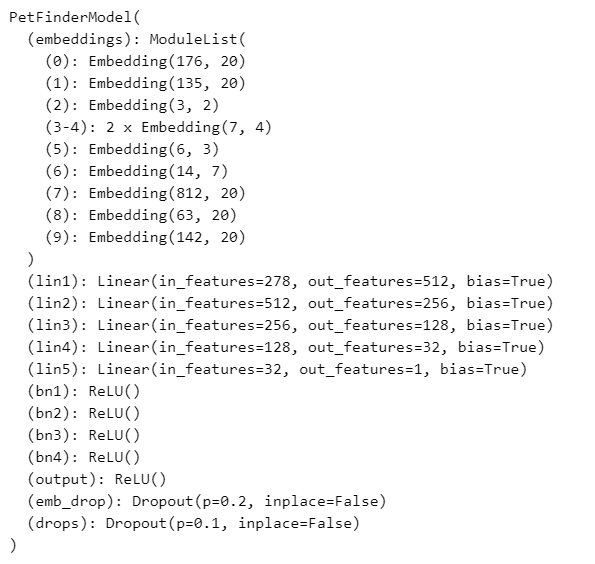
\includegraphics[width=0.7\textwidth]{Pictures/network.png}
        \caption{Network}
        \label{fig:network}
    \end{figure}
}
\end{frame}

\section{(Very Preliminary) Results}
\begin{frame}{(Very Preliminary) Results}
\only<1>{
\framesubtitle{Loss}
\begin{figure}
    \centering
    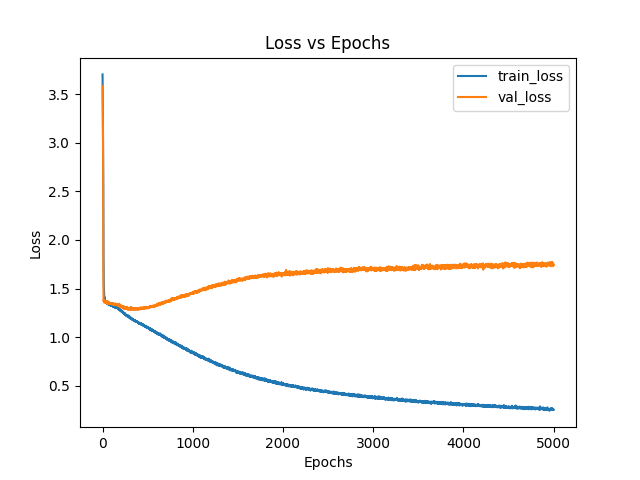
\includegraphics[width=0.8\textwidth]{Pictures/loss-stratify.png}
    \caption{Loss (Stratified)}
    \label{fig:loss}
\end{figure}
}
\only<2>{
\framesubtitle{Weighted Kappa}
\begin{figure}
    \centering
    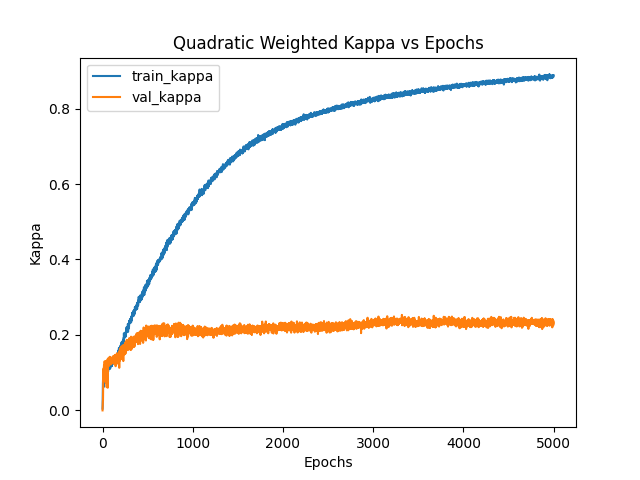
\includegraphics[width=0.8\textwidth]{Pictures/kappa-stratify.png}
    \caption{Kappa (Stratified)}
    \label{fig:kappa}
\end{figure}
}
\end{frame}